\title{MATR 200A HW1}
\author{John Goiri}
\date{\today}


\documentclass[12pt, fleqn]{article}
\usepackage{amsmath}
\usepackage{graphicx}
\usepackage{sidecap}
\usepackage{multicol}
\usepackage[small]{caption}
\usepackage{amsfonts}
\usepackage{breqn}
\usepackage[export]{adjustbox}

\renewcommand{\thesubsection}{\thesection.\alph{subsection}}
\renewcommand{\thesubsubsection}{\thesubsection.\alph{subsubsection}}
\begin{document}

\section{Point group of triangular lattice}
The basis vectors of a triangular lattice are $\vec{a}=\hat{i}+0\hat{j}$
and $\vec{b}=\frac{1}{2}\hat{i}+\frac{\sqrt{3}}{2}\hat{j}$.

\begin{figure}[h]
    \begin{center}
        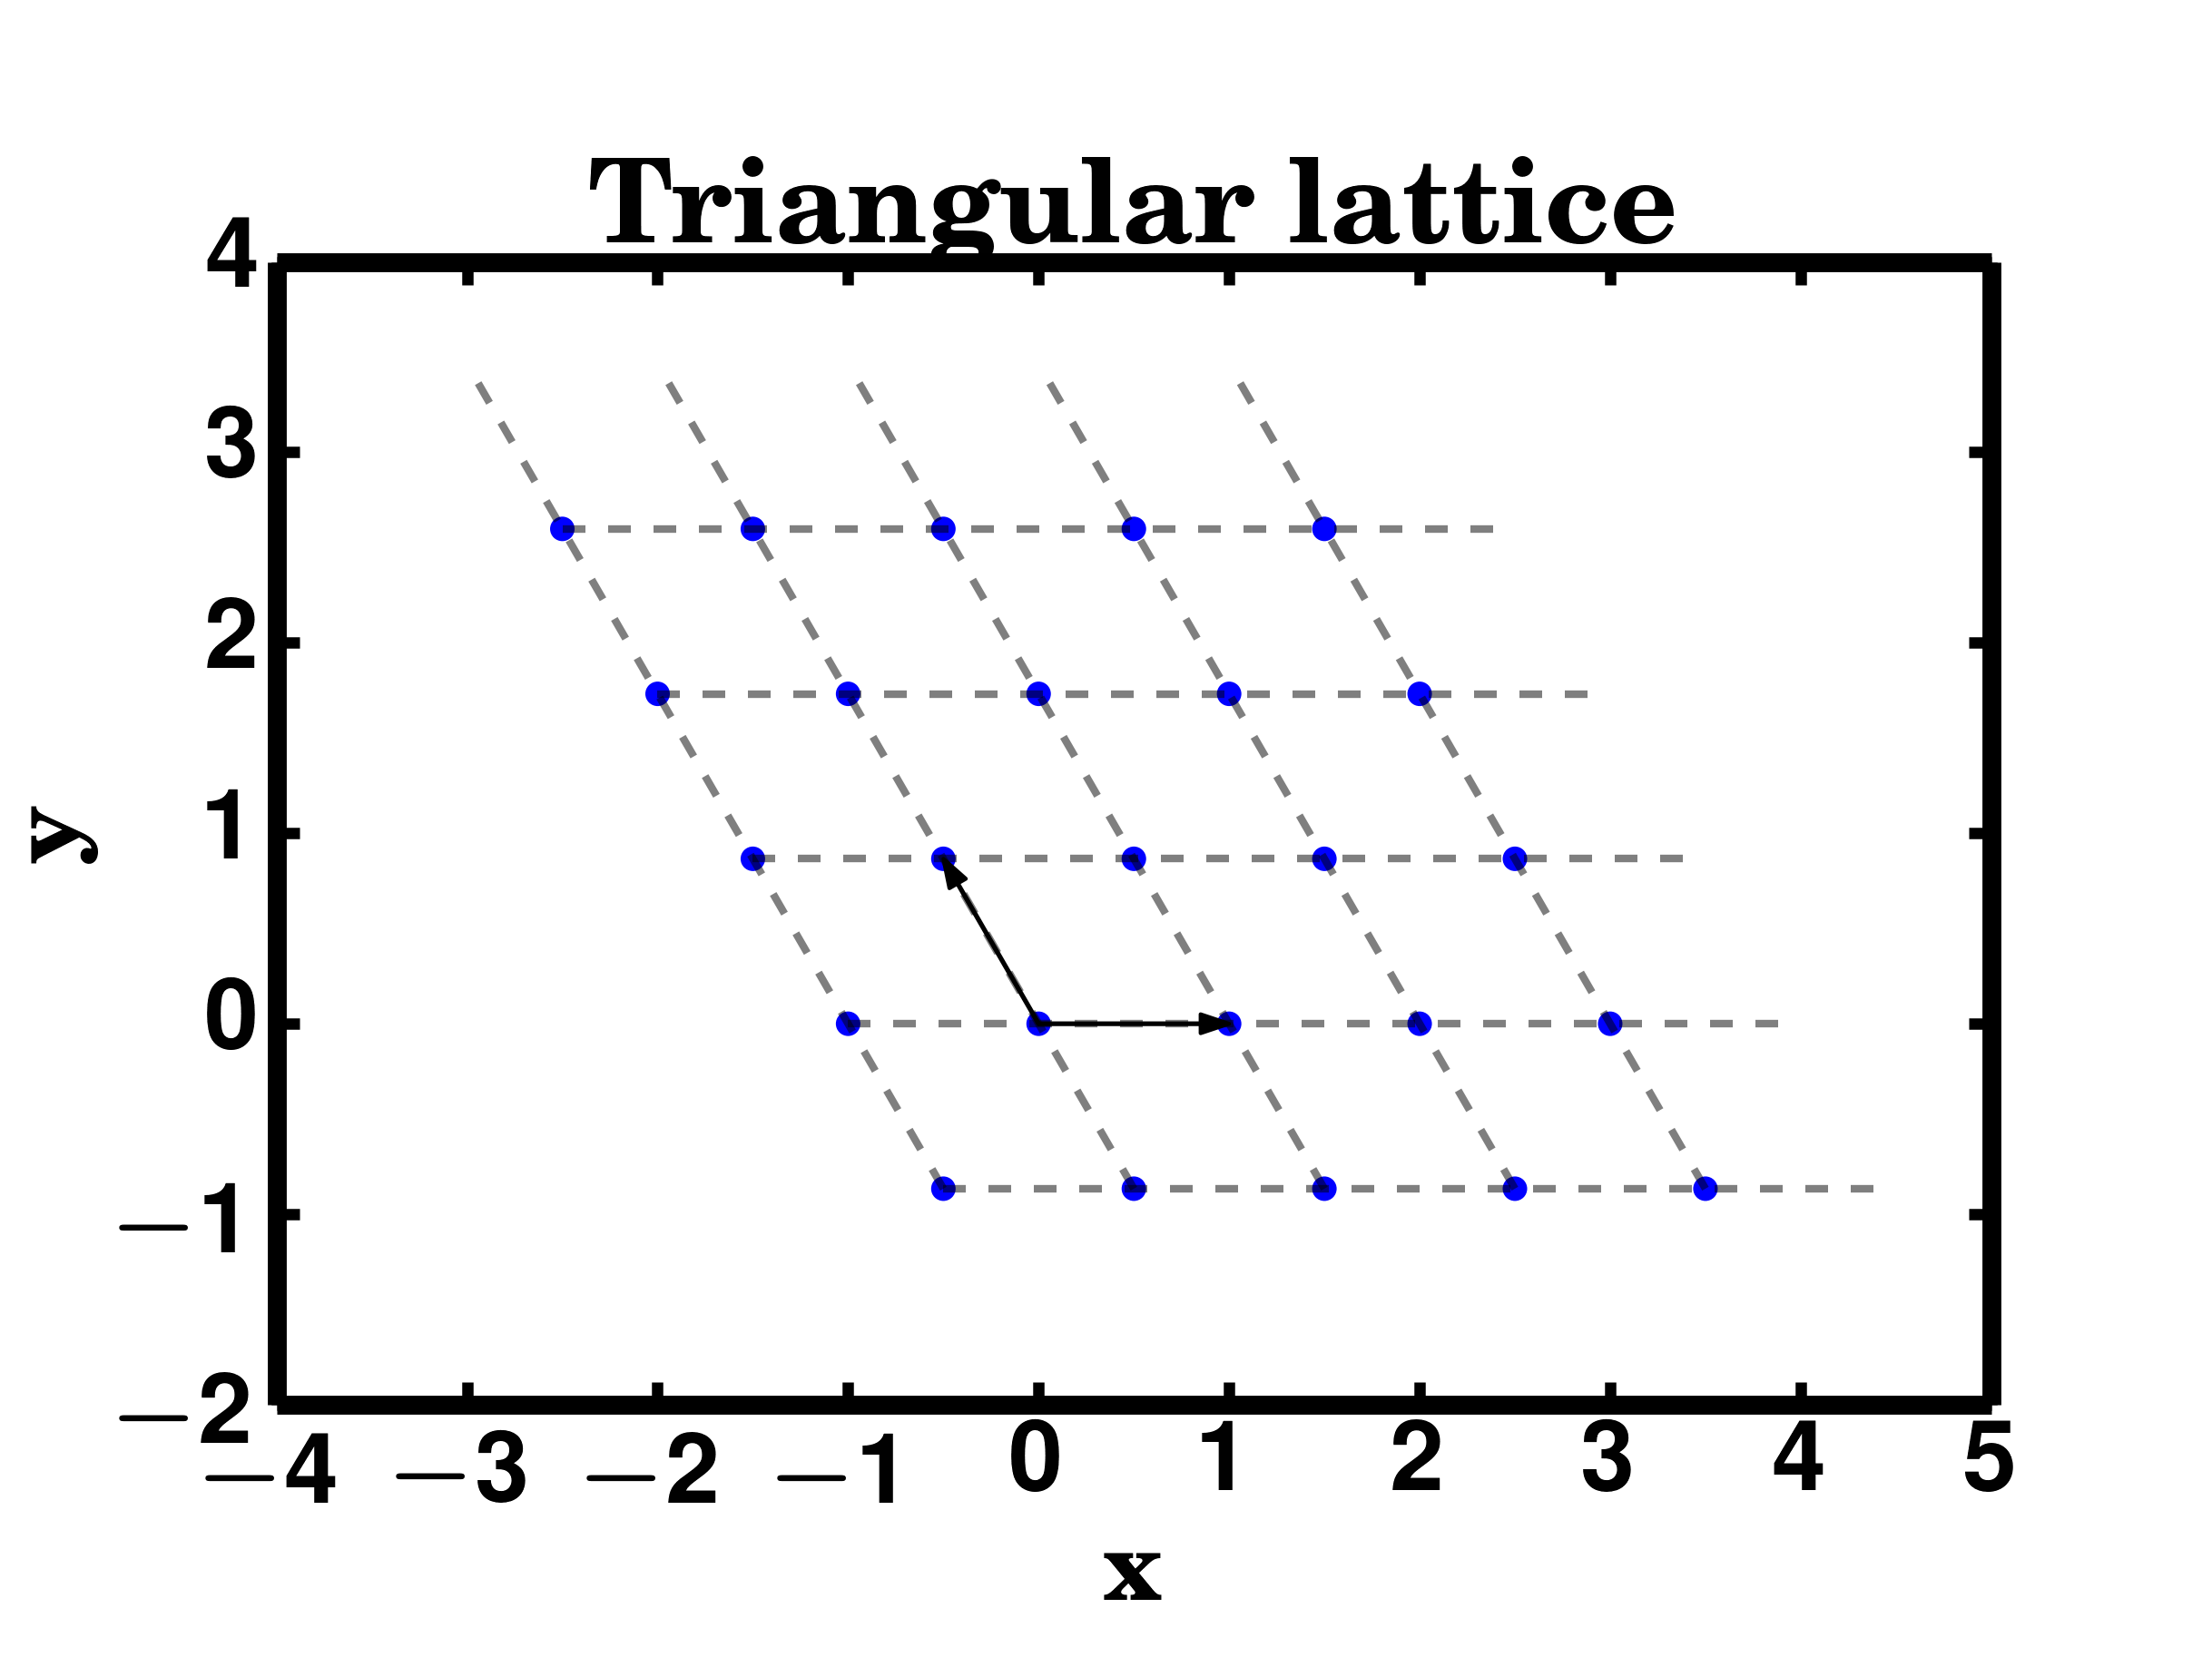
\includegraphics[max width=\textwidth]{./triangular.png}
    \end{center}
    \caption{Repeated basis vectors of a triangular lattice}
    \label{fig:triangular}
\end{figure}

This lattice has a total of 12 symmetry operations:

I0
\begin{equation}
    S=
    \begin{pmatrix}
        1.0&0.0\\
        0.0&1.0
    \end{pmatrix}
    ,\vec{\tau}=
    \begin{pmatrix}
        0\\
        0
    \end{pmatrix}
    \label{I0}
\end{equation}

R60
\begin{equation}
    S=
    \begin{pmatrix}
        0.5&-\frac{\sqrt{3}}{2}\\
        \frac{\sqrt{3}}{2}&0.5
    \end{pmatrix}
    ,\vec{\tau}=
    \begin{pmatrix}
        0\\
        0
    \end{pmatrix}
    \label{R60}
\end{equation}

R120
\begin{equation}
    S=
    \begin{pmatrix}
        -0.5&-\frac{\sqrt{3}}{2}\\
        \frac{\sqrt{3}}{2}&-0.5
    \end{pmatrix}
    ,\vec{\tau}=
    \begin{pmatrix}
        0\\
        0
    \end{pmatrix}
    \label{R120}
\end{equation}

R180
\begin{equation}
    S=
    \begin{pmatrix}
        -1.0&0.0\\
        0.0&-1.0
    \end{pmatrix}
    ,\vec{\tau}=
    \begin{pmatrix}
        0\\
        0
    \end{pmatrix}
    \label{R180}
\end{equation}

R240
\begin{equation}
    S=
    \begin{pmatrix}
        -0.5&\frac{\sqrt{3}}{2}\\
        -\frac{\sqrt{3}}{2}&-0.5
    \end{pmatrix}
    ,\vec{\tau}=
    \begin{pmatrix}
        0\\
        0
    \end{pmatrix}
    \label{R240}
\end{equation}

R300
\begin{equation}
    S=
    \begin{pmatrix}
        0.5&\frac{\sqrt{3}}{2}\\
        -\frac{\sqrt{3}}{2}&0.5
    \end{pmatrix}
    ,\vec{\tau}=
    \begin{pmatrix}
        0\\
        0
    \end{pmatrix}
    \label{R300}
\end{equation}

M0
\begin{equation}
    S=
    \begin{pmatrix}
        1.0&0.0\\
        0.0&-1.0
    \end{pmatrix}
    ,\vec{\tau}=
    \begin{pmatrix}
        0\\
        0
    \end{pmatrix}
    \label{M0}
\end{equation}

M30
\begin{equation}
    S=
    \begin{pmatrix}
        0.5&\frac{\sqrt{3}}{2}\\
        \frac{\sqrt{3}}{2}&-0.5
    \end{pmatrix}
    ,\vec{\tau}=
    \begin{pmatrix}
        0\\
        0
    \end{pmatrix}
    \label{M30}
\end{equation}

M60
\begin{equation}
    S=
    \begin{pmatrix}
        -0.5&\frac{\sqrt{3}}{2}\\
        \frac{\sqrt{3}}{2}&0.5
    \end{pmatrix}
    ,\vec{\tau}=
    \begin{pmatrix}
        0\\
        0
    \end{pmatrix}
    \label{M60}
\end{equation}

M90
\begin{equation}
    S=
    \begin{pmatrix}
        -1.0&0.0\\
        0.0&1.0
    \end{pmatrix}
    ,\vec{\tau}=
    \begin{pmatrix}
        0\\
        0
    \end{pmatrix}
    \label{M90}
\end{equation}

M120
\begin{equation}
    S=
    \begin{pmatrix}
        -0.5&-\frac{\sqrt{3}}{2}\\
        -\frac{\sqrt{3}}{2}&0.5
    \end{pmatrix}
    ,\vec{\tau}=
    \begin{pmatrix}
        0\\
        0
    \end{pmatrix}
    \label{M120}
\end{equation}

M150
\begin{equation}
    S=
    \begin{pmatrix}
        0.5&-\frac{\sqrt{3}}{2}\\
        -\frac{\sqrt{3}}{2}&-0.5
    \end{pmatrix}
    ,\vec{\tau}=
    \begin{pmatrix}
        0\\
        0
    \end{pmatrix}
    \label{M150}
\end{equation}

We can verify that it forms a closed group by combining every operation with another and
realizing the resulting operation is already part of the group.

\begin{table}[h!]
    \centering
    \resizebox{\columnwidth}{!}{%
    \centering
    \begin{tabular}{ l l l l l l l l l l l l }
        I0      &R60     &R120    &R180    &R240    &R300    &M0      &M30     &M60     &M90     &M120    &M150 \\ 
        R60     &R120    &R180    &R240    &R300    &I0      &M30     &M60     &M90     &M120    &M150    &M0   \\ 
        R120    &R180    &R240    &R300    &I0      &R60     &M60     &M90     &M120    &M150    &M0      &M30  \\ 
        R180    &R240    &R300    &I0      &R60     &R120    &M90     &M120    &M150    &M0      &M30     &M60  \\ 
        R240    &R300    &I0      &R60     &R120    &R180    &M120    &M150    &M0      &M30     &M60     &M90  \\ 
        R300    &I0      &R60     &R120    &R180    &R240    &M150    &M0      &M30     &M60     &M90     &M120 \\ 
        M0      &M150    &M120    &M90     &M60     &M30     &I0      &R300    &R240    &R180    &R120    &R60  \\ 
        M30     &M0      &M150    &M120    &M90     &M60     &R60     &I0      &R300    &R240    &R180    &R120 \\ 
        M60     &M30     &M0      &M150    &M120    &M90     &R120    &R60     &I0      &R300    &R240    &R180 \\ 
        M90     &M60     &M30     &M0      &M150    &M120    &R180    &R120    &R60     &I0      &R300    &R240 \\ 
        M120    &M90     &M60     &M30     &M0      &M150    &R240    &R180    &R120    &R60     &I0      &R300 \\ 
        M150    &M120    &M90     &M60     &M30     &M0      &R300    &R240    &R180    &R120    &R60     &I0   \\ 
    \end{tabular}
    }
    \caption{Multiplication table for the point group of a triangular lattice}
    \label{tab:mult}
\end{table}

\newpage
\section{Factor group of honeycomb lattice}
The honeycomb structure has the same lattice vectors as the triangular lattice, but two basis atoms.

\begin{figure}[h]
    \begin{center}
        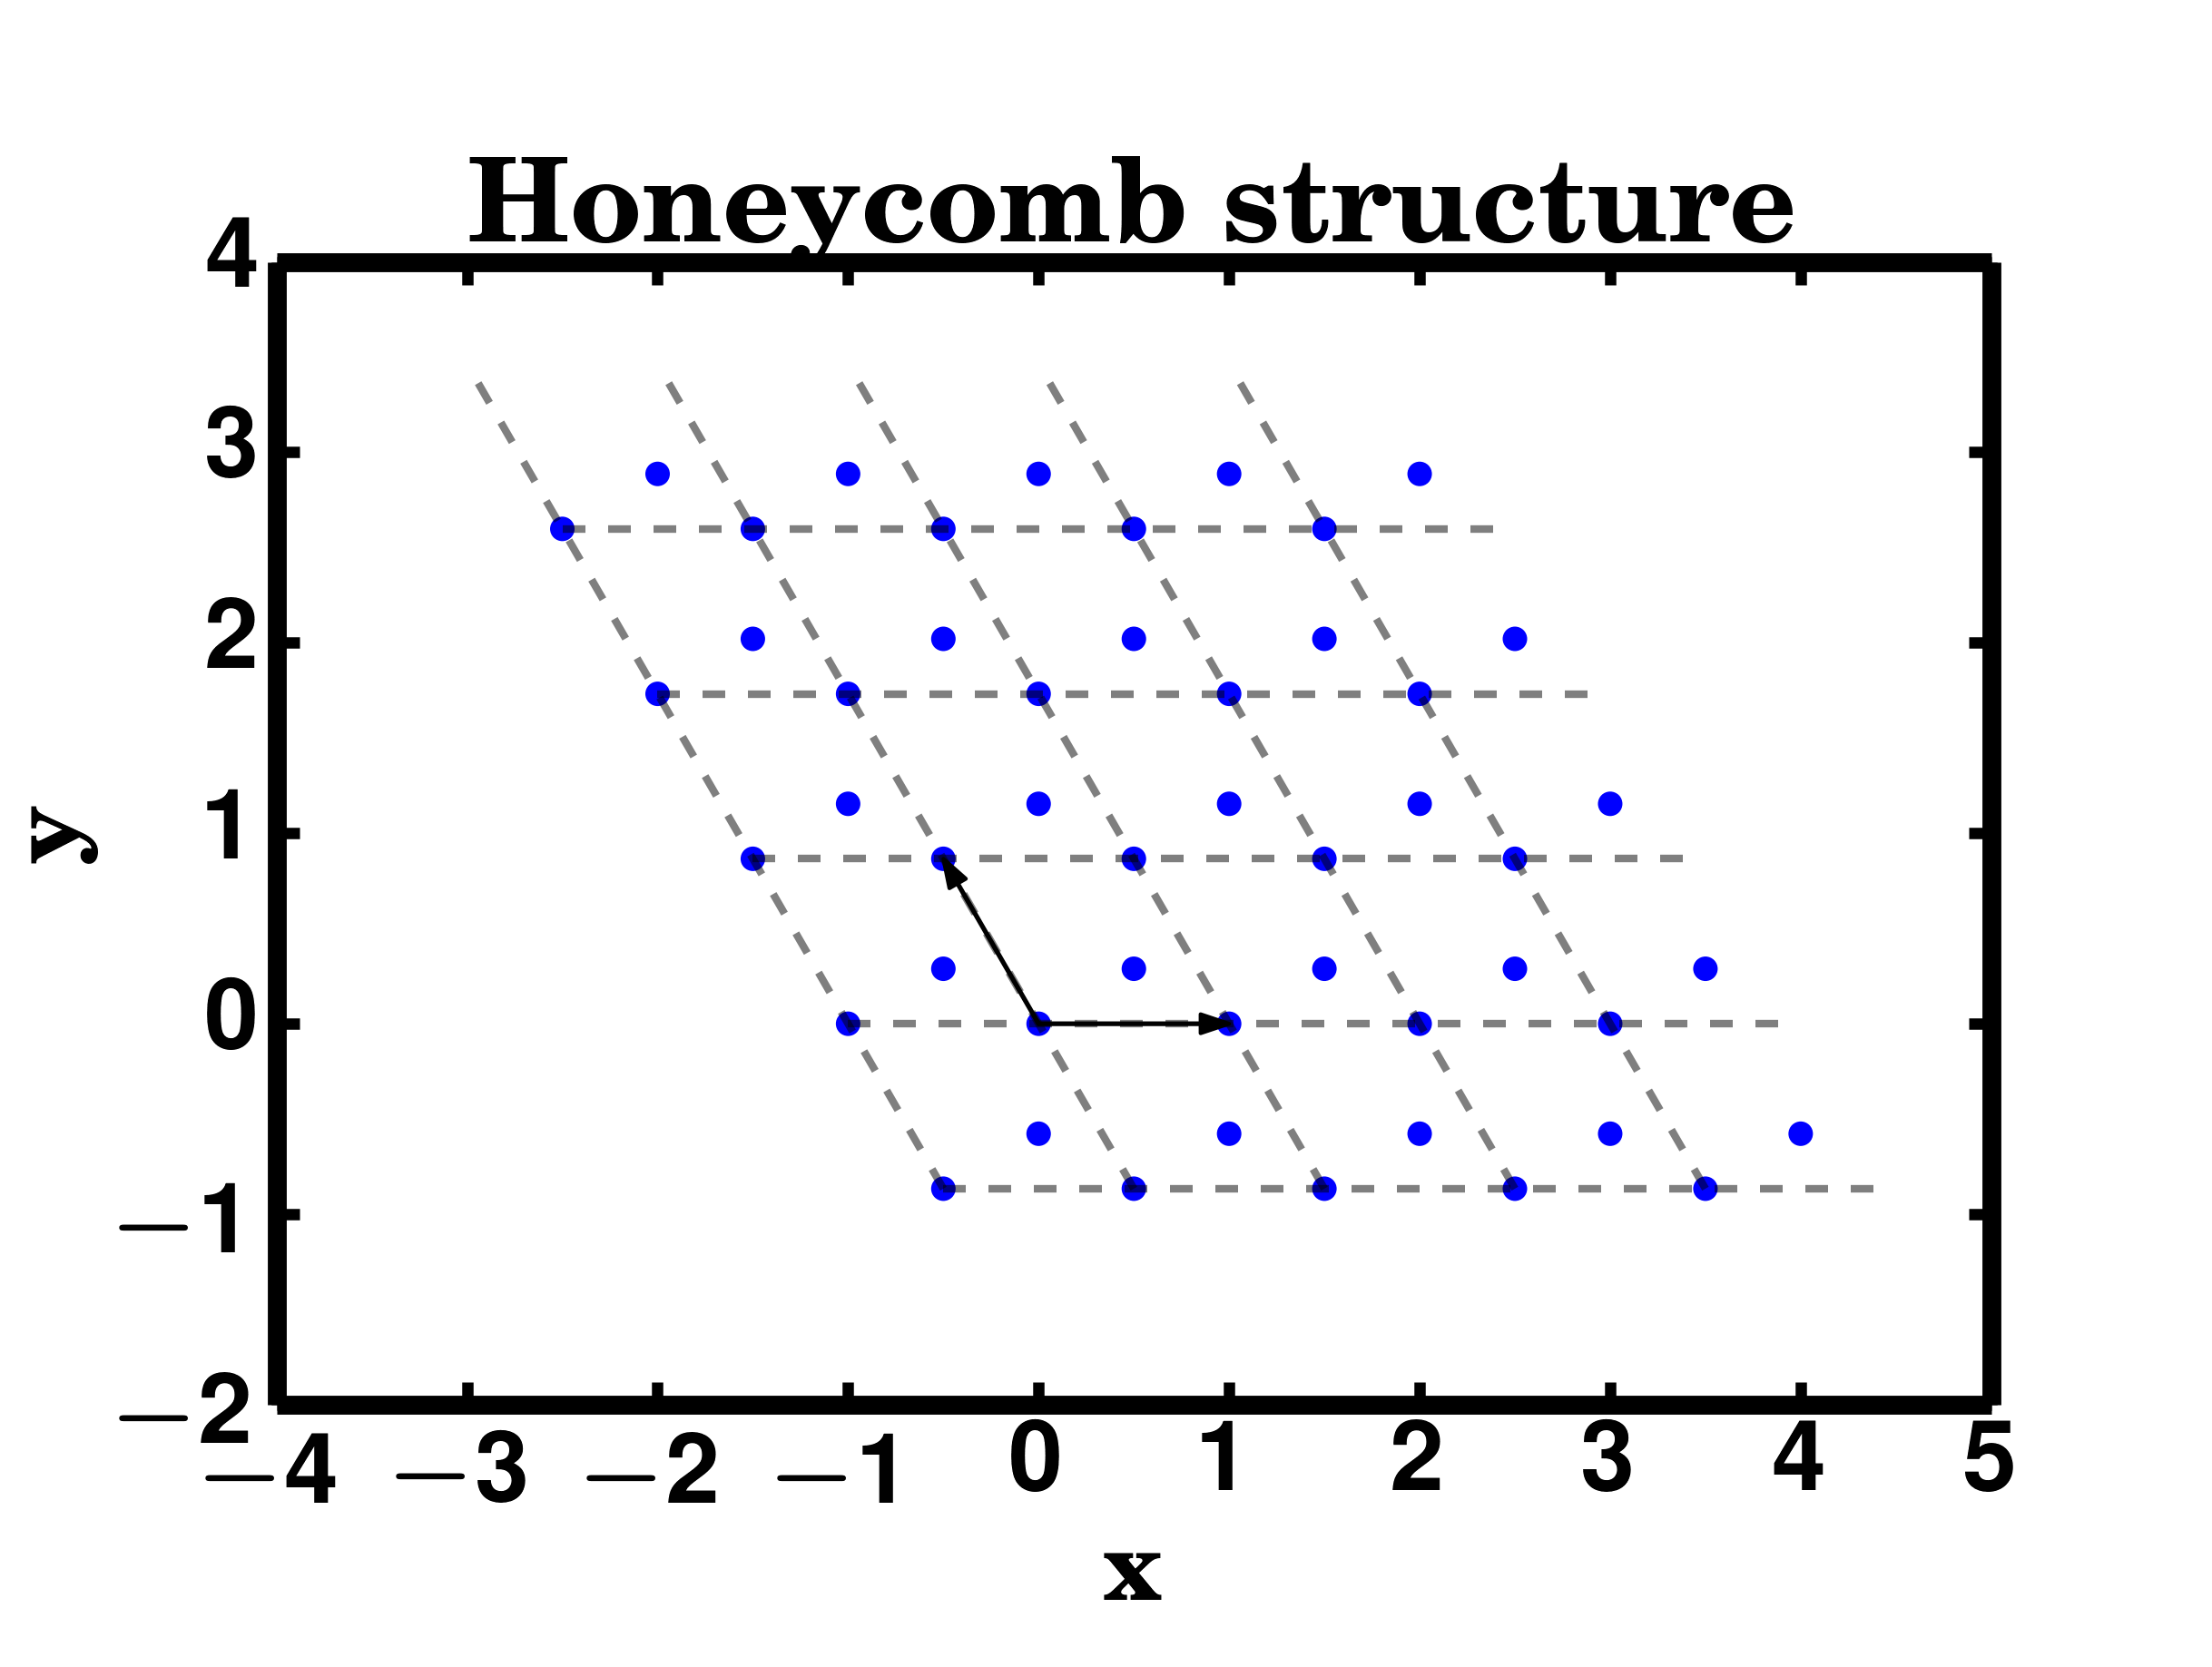
\includegraphics[max width=\textwidth]{./honeycomb.png}
    \end{center}
    \caption{Repeated basis vectors of a triangular lattice}
    \label{fig:honey}
\end{figure}

The factor group for this structure is the same as the point group, with half operations involving a translation.

I0
\begin{equation}
    S=
    \begin{pmatrix}
        1.0&0.0\\
        0.0&1.0
    \end{pmatrix}
    ,\vec{\tau}=
    \begin{pmatrix}
        0.0\\
        0.0
    \end{pmatrix}
    \label{I0}
\end{equation}

R60
\begin{equation}
    S=
    \begin{pmatrix}
        0.5&-\frac{\sqrt{3}}{2}\\
        \frac{\sqrt{3}}{2}&0.5
    \end{pmatrix}
    ,\vec{\tau}=
    \begin{pmatrix}
        0.5\\
        \frac{\sqrt{3}}{6}
    \end{pmatrix}
    \label{R60}
\end{equation}

R120
\begin{equation}
    S=
    \begin{pmatrix}
        -0.5&-\frac{\sqrt{3}}{2}\\
        \frac{\sqrt{3}}{2}&-0.5
    \end{pmatrix}
    ,\vec{\tau}=
    \begin{pmatrix}
        0.0\\
        0.0
    \end{pmatrix}
    \label{R120}
\end{equation}

R180
\begin{equation}
    S=
    \begin{pmatrix}
        -1.0&0.0\\
        0.0&-1.0
    \end{pmatrix}
    ,\vec{\tau}=
    \begin{pmatrix}
        0.5\\
        \frac{\sqrt{3}}{6}
    \end{pmatrix}
    \label{R180}
\end{equation}

R240
\begin{equation}
    S=
    \begin{pmatrix}
        -0.5&\frac{\sqrt{3}}{2}\\
        -\frac{\sqrt{3}}{2}&-0.5
    \end{pmatrix}
    ,\vec{\tau}=
    \begin{pmatrix}
        0.0\\
        0.0
    \end{pmatrix}
    \label{R240}
\end{equation}

R300
\begin{equation}
    S=
    \begin{pmatrix}
        0.5&\frac{\sqrt{3}}{2}\\
        -\frac{\sqrt{3}}{2}&0.5
    \end{pmatrix}
    ,\vec{\tau}=
    \begin{pmatrix}
        0.5\\
        \frac{\sqrt{3}}{6}
    \end{pmatrix}
    \label{R300}
\end{equation}

M0
\begin{equation}
    S=
    \begin{pmatrix}
        1.0&0.0\\
        0.0&-1.0
    \end{pmatrix}
    ,\vec{\tau}=
    \begin{pmatrix}
        0.5\\
        \frac{\sqrt{3}}{6}
    \end{pmatrix}
    \label{M0}
\end{equation}

M30
\begin{equation}
    S=
    \begin{pmatrix}
        0.5&\frac{\sqrt{3}}{2}\\
        \frac{\sqrt{3}}{2}&-0.5
    \end{pmatrix}
    ,\vec{\tau}=
    \begin{pmatrix}
        0.0\\
        0.0
    \end{pmatrix}
    \label{M30}
\end{equation}

M60
\begin{equation}
    S=
    \begin{pmatrix}
        -0.5&\frac{\sqrt{3}}{2}\\
        \frac{\sqrt{3}}{2}&0.5
    \end{pmatrix}
    ,\vec{\tau}=
    \begin{pmatrix}
        0.5\\
        \frac{\sqrt{3}}{6}
    \end{pmatrix}
    \label{M60}
\end{equation}

M90
\begin{equation}
    S=
    \begin{pmatrix}
        -1.0&0.0\\
        0.0&1.0
    \end{pmatrix}
    ,\vec{\tau}=
    \begin{pmatrix}
        0.0\\
        0.0
    \end{pmatrix}
    \label{M90}
\end{equation}

M120
\begin{equation}
    S=
    \begin{pmatrix}
        -0.5&-\frac{\sqrt{3}}{2}\\
        -\frac{\sqrt{3}}{2}&0.5
    \end{pmatrix}
    ,\vec{\tau}=
    \begin{pmatrix}
        0.5\\
        \frac{\sqrt{3}}{6}
    \end{pmatrix}
    \label{M120}
\end{equation}

M150
\begin{equation}
    S=
    \begin{pmatrix}
        0.5&-\frac{\sqrt{3}}{2}\\
        -\frac{\sqrt{3}}{2}&-0.5
    \end{pmatrix}
    ,\vec{\tau}=
    \begin{pmatrix}
        0.0\\
        0.0
    \end{pmatrix}
    \label{M150}
\end{equation}

\end{document}
